\chapter[Implementation ]{Research Implementation }
\vspace{5pt}

Implementation of this research can be divided mainly into three parts which are Ad-hoc network implementation, Cellular plane implementation, and Control plane implementation.
Let us consider those parts in detail.

\subsection{Ad-hoc Network Implementation}
Let us consider the ad-hoc network implementation. When implementing the ad-hoc network first we need to consider the Architecture of the Android OS. Android OS consists of the following components.
\begin{figure}[H]
    \centering
    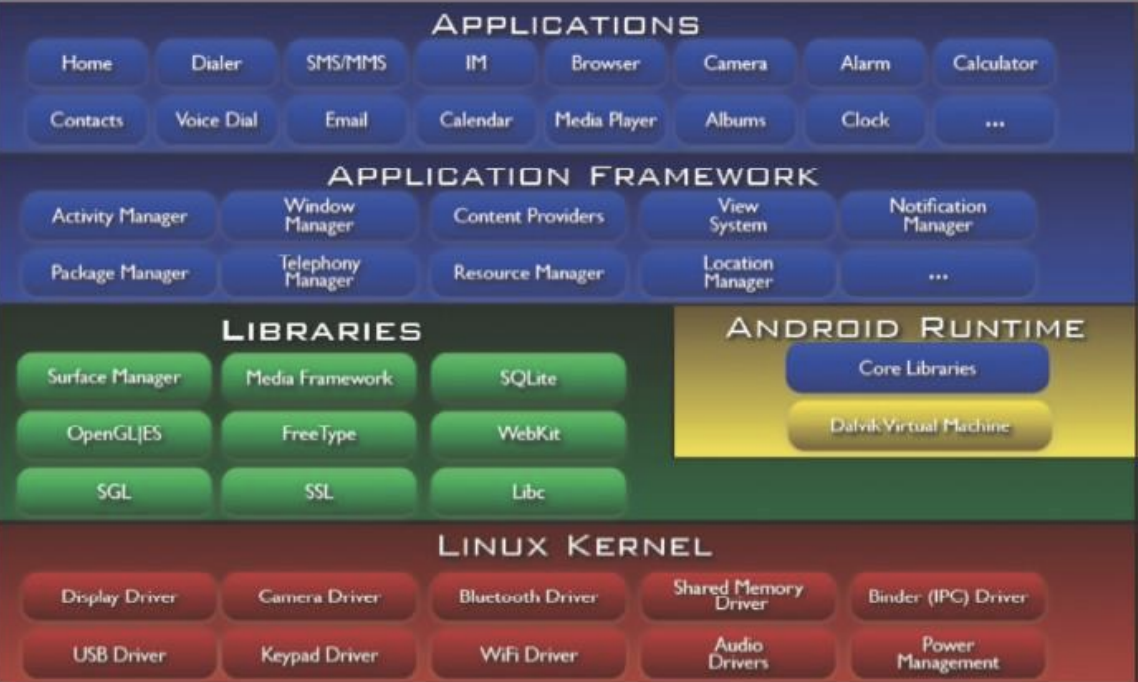
\includegraphics[scale=0.74]{system_archetecture}
    \caption{ Android system architecture. Green items are written in C/C++, blue
items are written in Java and run in the Dalvik VM.}
    \label{fig:pca_coeff_z_qws_12}
\end{figure}
\vspace{12pt}
\clearpage
When looking at the above architecture in Figure \ref{fig:pca_coeff_z_qws_12} we can see that there are three main choices to implement an ad -hoc network using an Android device. They are as follows.
\begin{enumerate}
  \item Implement the network on the Android OS layer 
  \item Implement the network inside the kernel module.
  \item Implement the network on the application level.
\end{enumerate}
\subsubsection{Implementing the network in the Android OS layer}
First, we tried to implement the ad-hoc network using the Android OS level by modifying the Java code. For this, we need a way to implement the ad-hoc networking stack in the OS layer components.

\vspace{5pt}
These components include network discovery module, IP assignment module. routing module and the control plane to orchestrate all of this. After trying to implement some of the modules it was evident to us that the time was not sufficient to finish the implementation. This is because Android OS takes a huge time to compile. It takes 16 thread 60Gb ram server about one and a half hours to compile the Android Open Source project. So with the available hardware and timeframe of one year, it was not feasible to go through this method.
\begin{figure}[H]
    \centering
    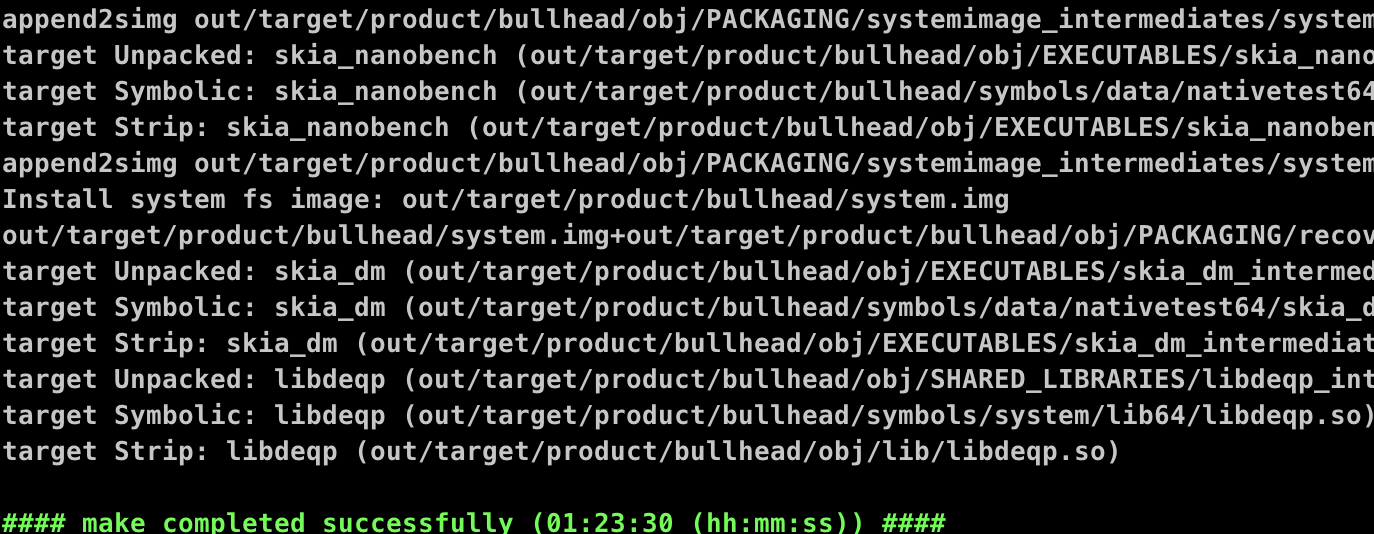
\includegraphics[scale=0.6]{aosp_compile_time}
    \caption{Image showing the time it takes to compile AOSP with the above-mentioned specs.}
\end{figure}
\vspace{12pt}
\clearpage
\subsubsection{Implementing the network inside the kernel module.}

The second option to enable ad-hoc networking in Android is to implement the whole system in the kernel layer. Due to the android kernel being derived from the Linux kernel it is easy to enable the batman routing protocol. To do this we need to recompile the kernel with the relevant modules enabled(B.A.T.M.A.N. module) and flash it back to the mobile device.

\begin{figure}[H]
    \centering
    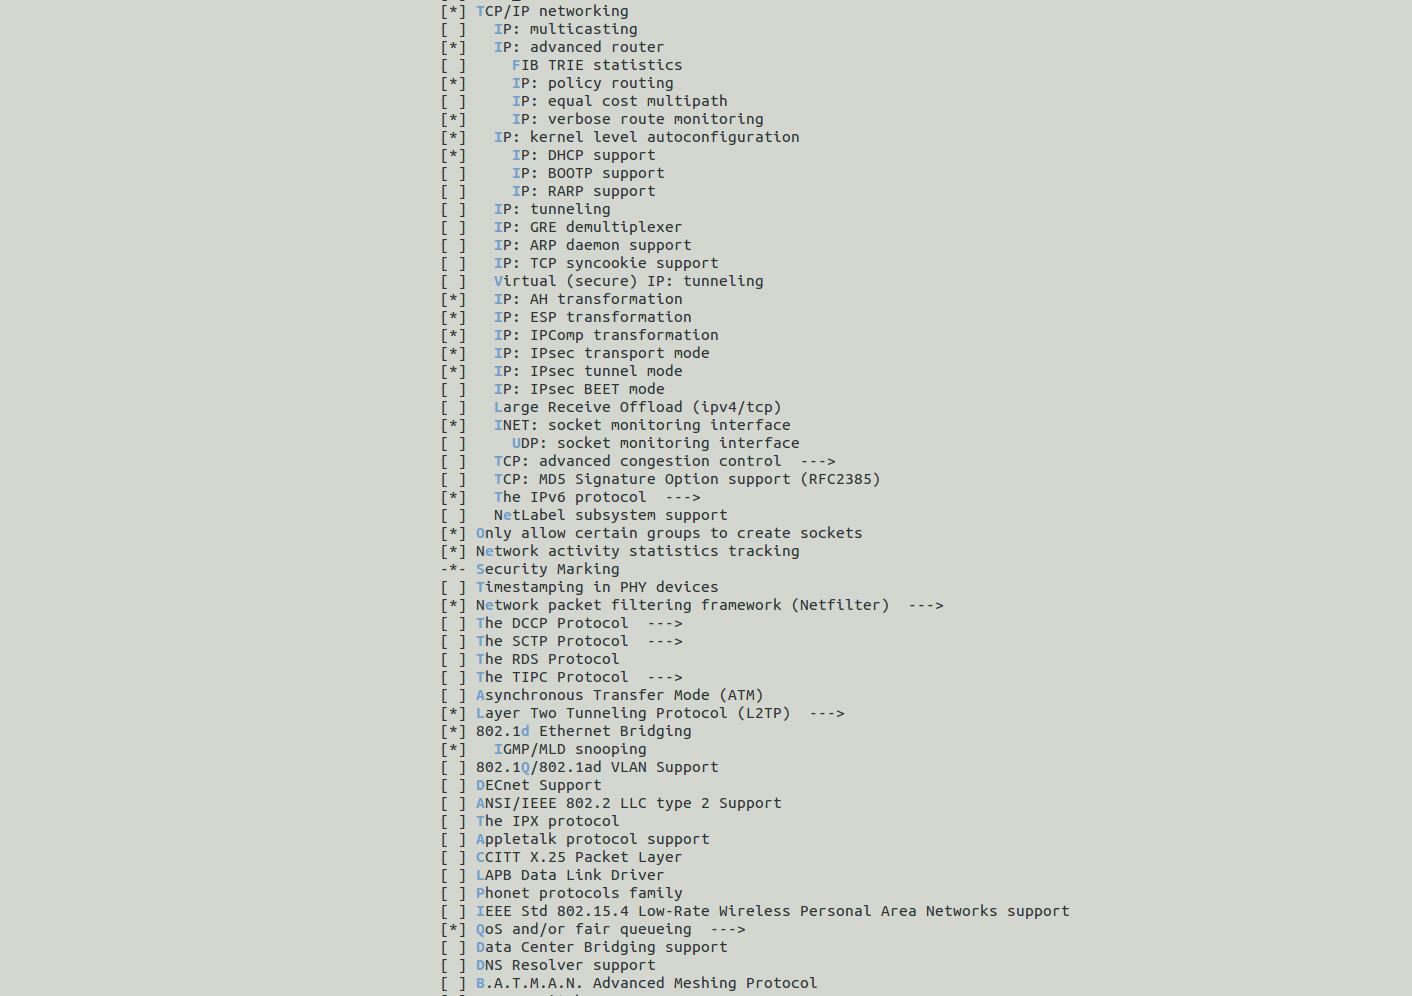
\includegraphics[scale=0.6]{andoid_kernel_defconfig}
    \caption{Android Kernel Default configuration}
    \label{fig:pca_df_dfgh_efege_fef_z}
\end{figure}
\vspace{12pt}
As you can see in the above Figure \ref{fig:pca_df_dfgh_efege_fef_z} default Android compilation setting does not include the most basic network drivers which are readily available to the general Linux kernel. So we need to enable those modules and recompile the Kernel to enable Ad-hoc features.
Doing this is kind of risky because if you flash a faulty kernel to the device it will brick the device. This is because the kernel for the android device is contained in its boot image. So if the boot process does not happen correctly there is no way to recover from that. Recovery mode and boot-loader mode needs the boot to function properly. As we did brick a test device it is not a safe method to implement the Ad-hoc network.

\clearpage


\subsubsection{Implement the network in the Application Layer}
After considering all the options we choose the application layer to implement the ad-hoc network because it is the best way to implement the network. 
Wi-Fi Direct (P2P) allows Android 4.0 (API level 14) or later devices with the appropriate hardware to connect directly to each other via Wi-Fi without any intermediate access point\cite{WiFiDirect_android}. Android implements the Wi-Fi Direct in accordance with the IEEE standard. So essentially this technology allows the Android developer to connect other devices using the Android built-in API.
\vspace{12pt}
\begin{figure}[H]
    \centering
    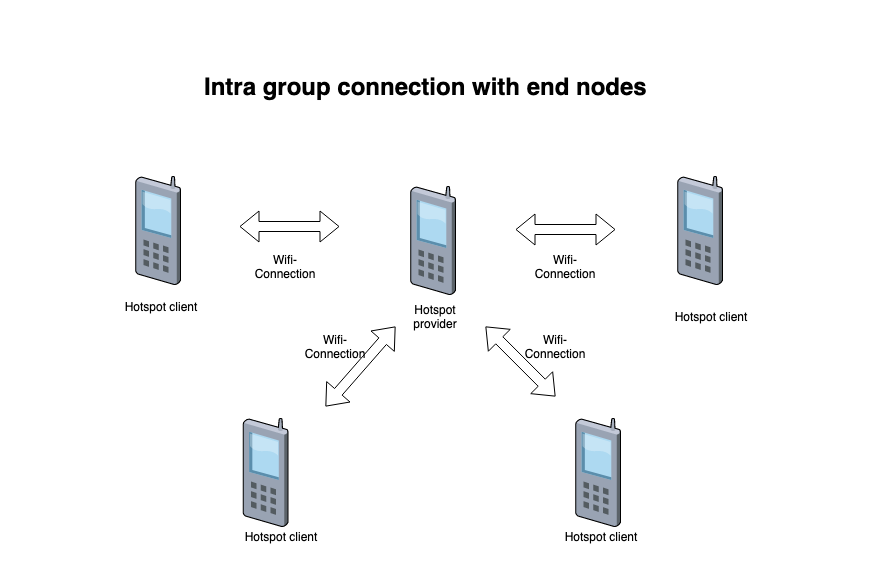
\includegraphics[scale=0.44]{images/Intra_group_communication}
    \caption{Wifi-direct group formation}
    \label{fig:timedffline_123_12_23}
\end{figure}

We created an application to connect the devices in the Wi-Fi Direct mode using this feature.
The application works in the following manner. Initial work() function starts the processes need for the application. First, it binds the GUI components like buttons tex boxes to the relevant variables. 


\begin{lstlisting}[language=Java]

private void initialWork() {
    btnOnOff=(Button) findViewById(R.id.onOff);
    btnDiscover=(Button) findViewById(R.id.discover);
    btnSend=(Button) findViewById(R.id.sendButton);
    listView=(ListView) findViewById(R.id.peerListView);
    read_msg_box=(TextView) findViewById(R.id.readMsg);
    connectionStatus=(TextView) findViewById(R.id.connectionStatus);
    writeMsg=(EditText) findViewById(R.id.writeMsg);}
\end{lstlisting}

To access the system WIFI service we need to bind the WIFI service to a wifiManager object. Then we need a channel to initialize the receiver object. This part happens in the following code segment.

\begin{lstlisting}[language=Java]
wifiManager= (WifiManager) getApplicationContext().getSystemService(Context.WIFI_SERVICE);

mManager= (WifiP2pManager) getSystemService(Context.WIFI_P2P_SERVICE);
mChannel=mManager.initialize(this,getMainLooper(),null);	
mReceiver=new WiFiDirectBroadcastReceiver(mManager, mChannel,this);
\end{lstlisting}
We need to create an intent filter object with the relevant permissions in order to get the privileges needed from the user..
\begin{lstlisting}[language=Java]
    mIntentFilter=new IntentFilter();
    mIntentFilter.addAction(WifiP2pManager.WIFI_P2P_STATE_CHANGED_ACTION);
    mIntentFilter.addAction(WifiP2pManager.WIFI_P2P_PEERS_CHANGED_ACTION);
    mIntentFilter.addAction(WifiP2pManager.WIFI_P2P_CONNECTION_CHANGED_ACTION);
    mIntentFilter.addAction(WifiP2pManager.WIFI_P2P_THIS_DEVICE_CHANGED_ACTION);
	
\end{lstlisting}

The Lambda function below is responsible for creating available WIFI Direct devices to be connected. It first clears the list at the beginning and then adds the devices by calling peerList.getDeviceList() method. The for-loop creates a device name list which is used to create the UI device list. If there is no device to connect it gives a toast stating no device found.  

\begin{lstlisting}[language=Java]
    WifiP2pManager.PeerListListener peerListListener=new WifiP2pManager.PeerListListener() {
        @Override
        public void onPeersAvailable(WifiP2pDeviceList peerList) {
            if(!peerList.getDeviceList().equals(peers))
            {
                peers.clear();
                peers.addAll(peerList.getDeviceList());

                deviceNameArray=new String[peerList.getDeviceList().size()];
                deviceArray=new WifiP2pDevice[peerList.getDeviceList().size()];
                int index=0;

                for(WifiP2pDevice device : peerList.getDeviceList())
                {
                    deviceNameArray[index]=device.deviceName;
                    deviceArray[index]=device;
                    index++;
                }

                ArrayAdapter<String> adapter=new ArrayAdapter<String>(getApplicationContext(),
                android.R.layout.simple_list_item_1,deviceNameArray);
                listView.setAdapter(adapter);
            }
            if(peers.size()==0)
            {
                Toast.makeText(getApplicationContext(),"No Device Found",Toast.LENGTH_SHORT).show();
                return;
            }
        }
    };
	
\end{lstlisting}

The below anonymous inner class differentiates the group owner from the client and provides the group security key for connecting the devices that support the WIFI protocol.

\begin{lstlisting}[language=Java]
WifiP2pManager.ConnectionInfoListener connectionInfoListener=new WifiP2pManager.ConnectionInfoListener() {
     @Override
     public void onConnectionInfoAvailable(WifiP2pInfo wifiP2pInfo) {
        final InetAddress groupOwnerAddress=wifiP2pInfo.groupOwnerAddress;
        final boolean isClient = !wifiP2pInfo.isGroupOwner;
        
        if(wifiP2pInfo.groupFormed && wifiP2pInfo.isGroupOwner){
            connectionStatus.setText(password+groupOwnerAddress.toString());
            serverClass=new ServerClass();
            serverClass.start();
        }else if(wifiP2pInfo.groupFormed){
            connectionStatus.setText("Client");
            clientClass=new ClientClass(groupOwnerAddress);
            clientClass.start();
         }}};	
\end{lstlisting}
Public method onReceive implement the logic that needed in connecting the two devices and provide the relevant toast message inform the state.

\begin{lstlisting}[language=Java]
public void onReceive(Context context, Intent intent) {
String action = intent.getAction();

if(WifiP2pManager.WIFI_P2P_STATE_CHANGED_ACTION.equals(action)){
    int state=intent.getIntExtra(WifiP2pManager.EXTRA_WIFI_STATE,-1);

    if(state==WifiP2pManager.WIFI_P2P_STATE_ENABLED){
        Toast.makeText(context,"Wifi is ON",Toast.LENGTH_SHORT).show();
    }else {
        Toast.makeText(context,"Wifi is OFF",Toast.LENGTH_SHORT).show();
    }
}else if(WifiP2pManager.WIFI_P2P_PEERS_CHANGED_ACTION.equals(action)){
    //do something
    if(mManager!=null)
    {
        mManager.requestPeers(mChannel,mActivity.peerListListener);
    }
}else if(WifiP2pManager.WIFI_P2P_CONNECTION_CHANGED_ACTION.equals(action)){
    //do something
    if(mManager==null)
    {
        return;
    }

    NetworkInfo networkInfo=intent.getParcelableExtra(WifiP2pManager.EXTRA_NETWORK_INFO);

    if(networkInfo.isConnected())
    {
        mManager.requestConnectionInfo(mChannel,mActivity.connectionInfoListener);
    }else {
        mActivity.connectionStatus.setText("Device Disconnected");
    }
}else if(WifiP2pManager.WIFI_P2P_THIS_DEVICE_CHANGED_ACTION.equals(action)){
	} 	
}
	
\end{lstlisting}
The GUI of the WIFI Direct application is shown in the Figure \ref{fig:timeffline_34FSEFS_q1} below. Left device acts as the group owner while the other acts the client. we have implemented a simple message passing app in order to test the connectivity between the devices.
\begin{figure}[H]
    \centering
    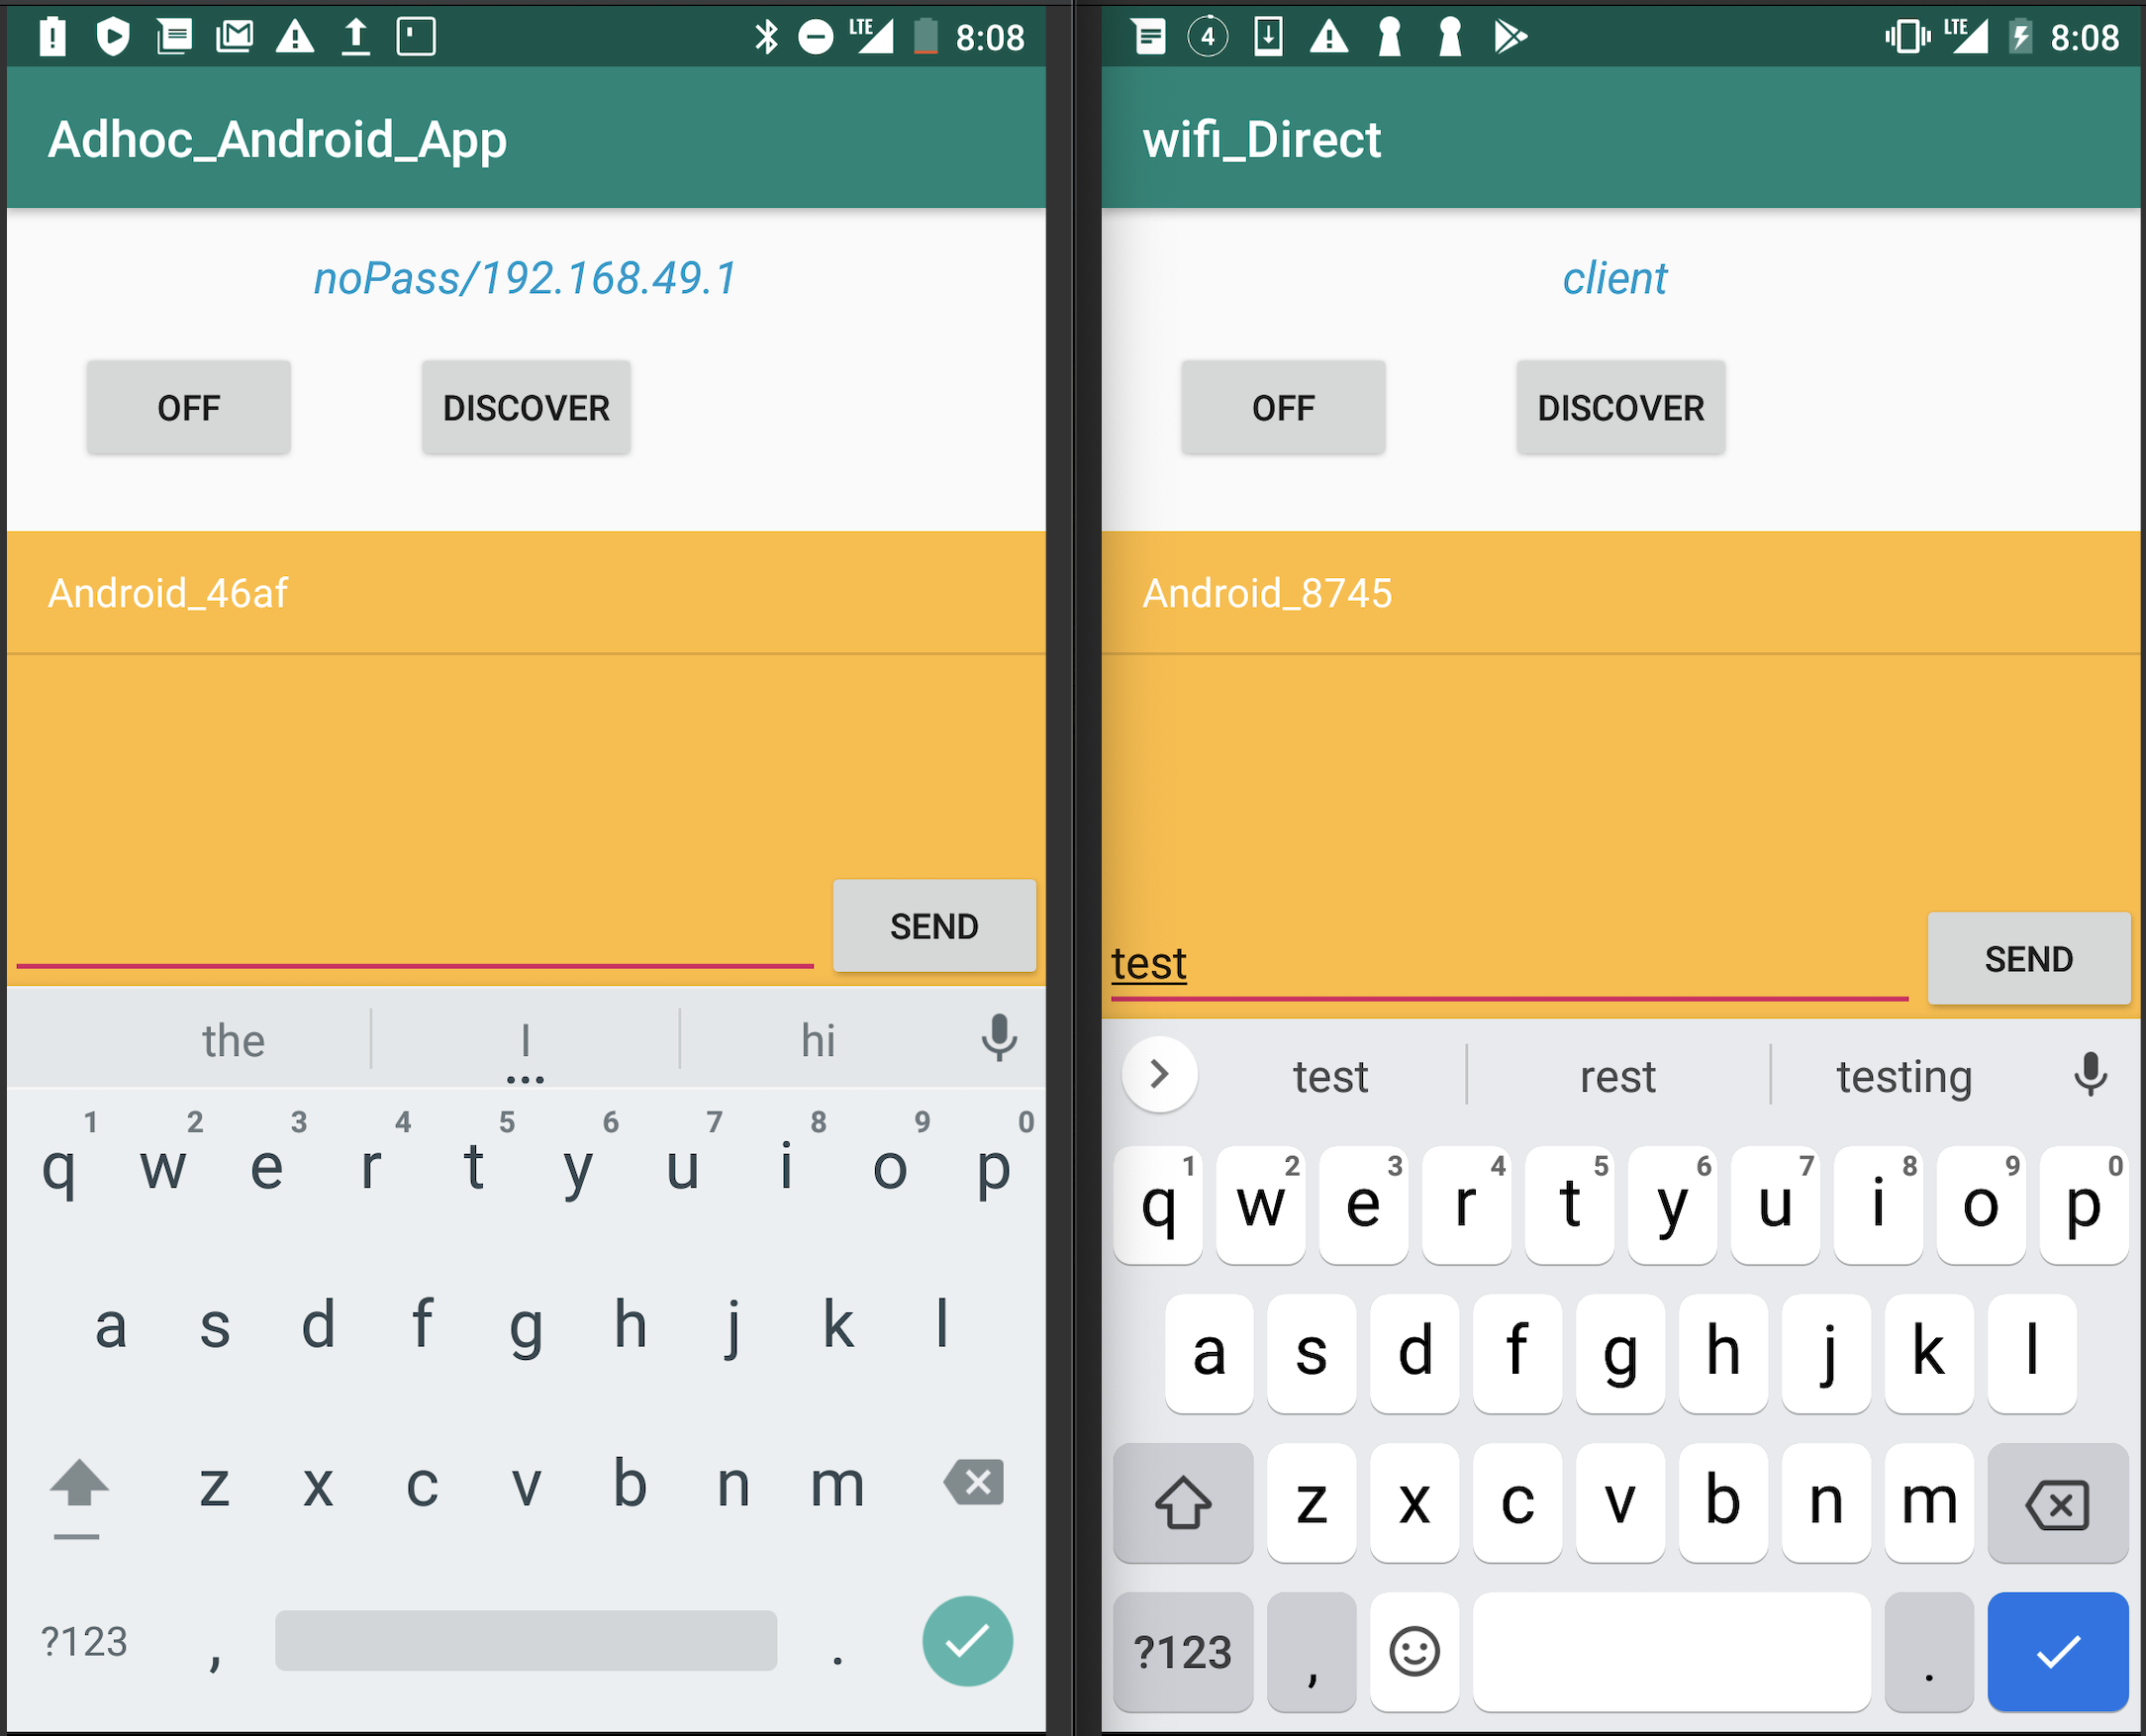
\includegraphics[scale=0.32]{gui_wifi_direct}
    \caption{GUI of the final version of WIFI Direct client}
    \label{fig:timeffline_34FSEFS_q1}
\end{figure}
\vspace{12pt}

When using the Android Wifi-direct implementation devices are provided with a hardcoded set of IP addresses. Due to this, there are limits to how many devices can be connected for a WIFI Direct group. We can mitigate this easily by modifying the AOSP code below to assign the IP address dynamically.
\begin{lstlisting}[language=Java]
    private static final String[] DHCP_RANGE = {"192.168.49.2", "192.168.49.254"};
    private static final String SERVER_ADDRESS = "192.168.49.1";	
\end{lstlisting}
Another option is to use the Android VPN connection to connect the android devices. With that, we can make the ad-hoc network using Wifi Direct protocol as follows.
and this provides the least modifications to the Android OS.

\begin{figure}[H]
    \centering
    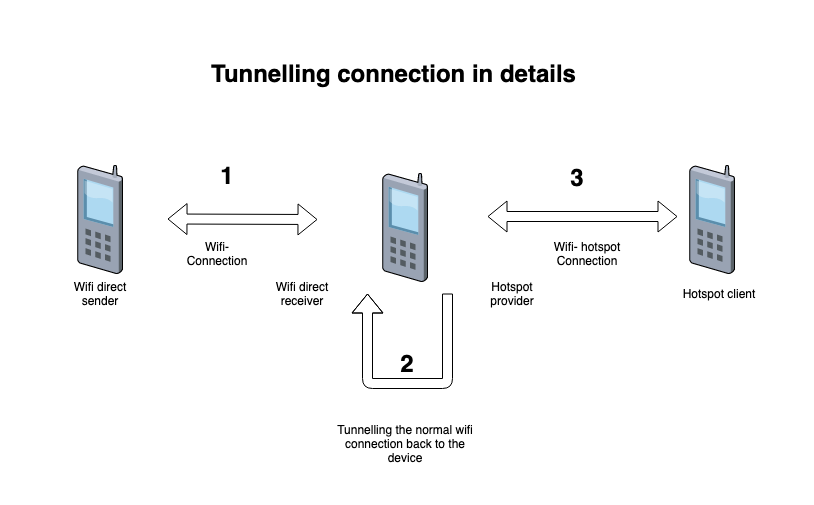
\includegraphics[scale=0.42]{images/tunnel_connection}
    \caption{How tunnel connections are used in the network for inter-cluster connections}
    \label{fig:timeffline_de_FR_W_AF_FW_FG_SDr}
\end{figure}
\vspace{12pt}
  


\subsection{Cellular Network Layar Implementation}

To work with the cellular network configuration we need good Linux networking tools like ifconfig, ip, tcpdump, and netstat with the driver support for their subcommands. The problem with working the Android OS is that it does not have any of these tools. And most of these tools need superuser execution privileges to work properly. Due to security concerns, Android OS does not provide superuser access for the users. So to do this we need to overcome these problems.
\subsubsection{Enabling the Root access for Android OS}
Android does not have superuser access by default so we need a way to implement that back to the android kernel. The easiest way is to modify the boot.img of the devices so that we can implement the root user. To do this first we need to add the su binary back to the source code. To create the su binary you need to cross-compile the source code with the correct cross compiler. In this case, it is aarch64-linux-android-4.9. 

Then we need to modify the initrd so that it spawns our custom process with the root privileges. Then we can use the privilege manager application like superSU to manage the root privileges via the custom initrd process. The actual process is much more complicated than the one we mentioned previously. 

\begin{figure}[H]
    \centering
    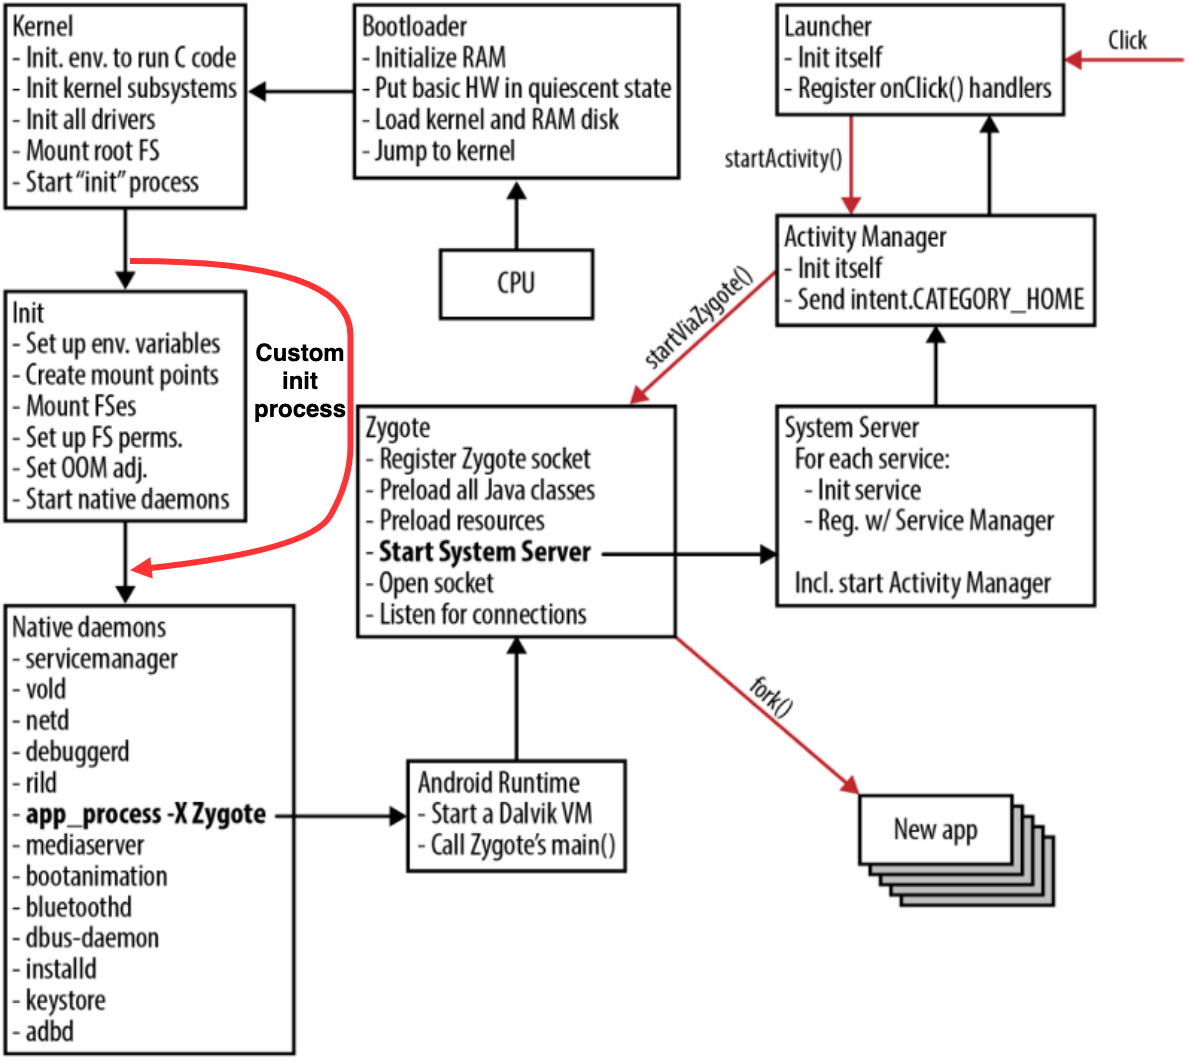
\includegraphics[scale=0.27]{boot_android_process}
    \caption{The boot process of Android}
    \label{fig:boot_android_process_d1212}
\end{figure}
\vspace{12pt}

\subsubsection{Porting the Networking tools to Android}

After successfully rooting the devices next we need the networking tools to call the kernel modules. For this, we tried the already available solution called busybox. This was not sufficient because it lacks some fundamental tools which are needed for implementing the network. So we used the ported version of the Debian package manager for this research. Fortunately, there was a ported version of the Debian package manager that was available in the termux\cite{termux} open source project. So we used the termux packages and their build scripts to cross-compile the networking tools to my test device Nexus 5x.
\begin{figure}[H]
    \centering
    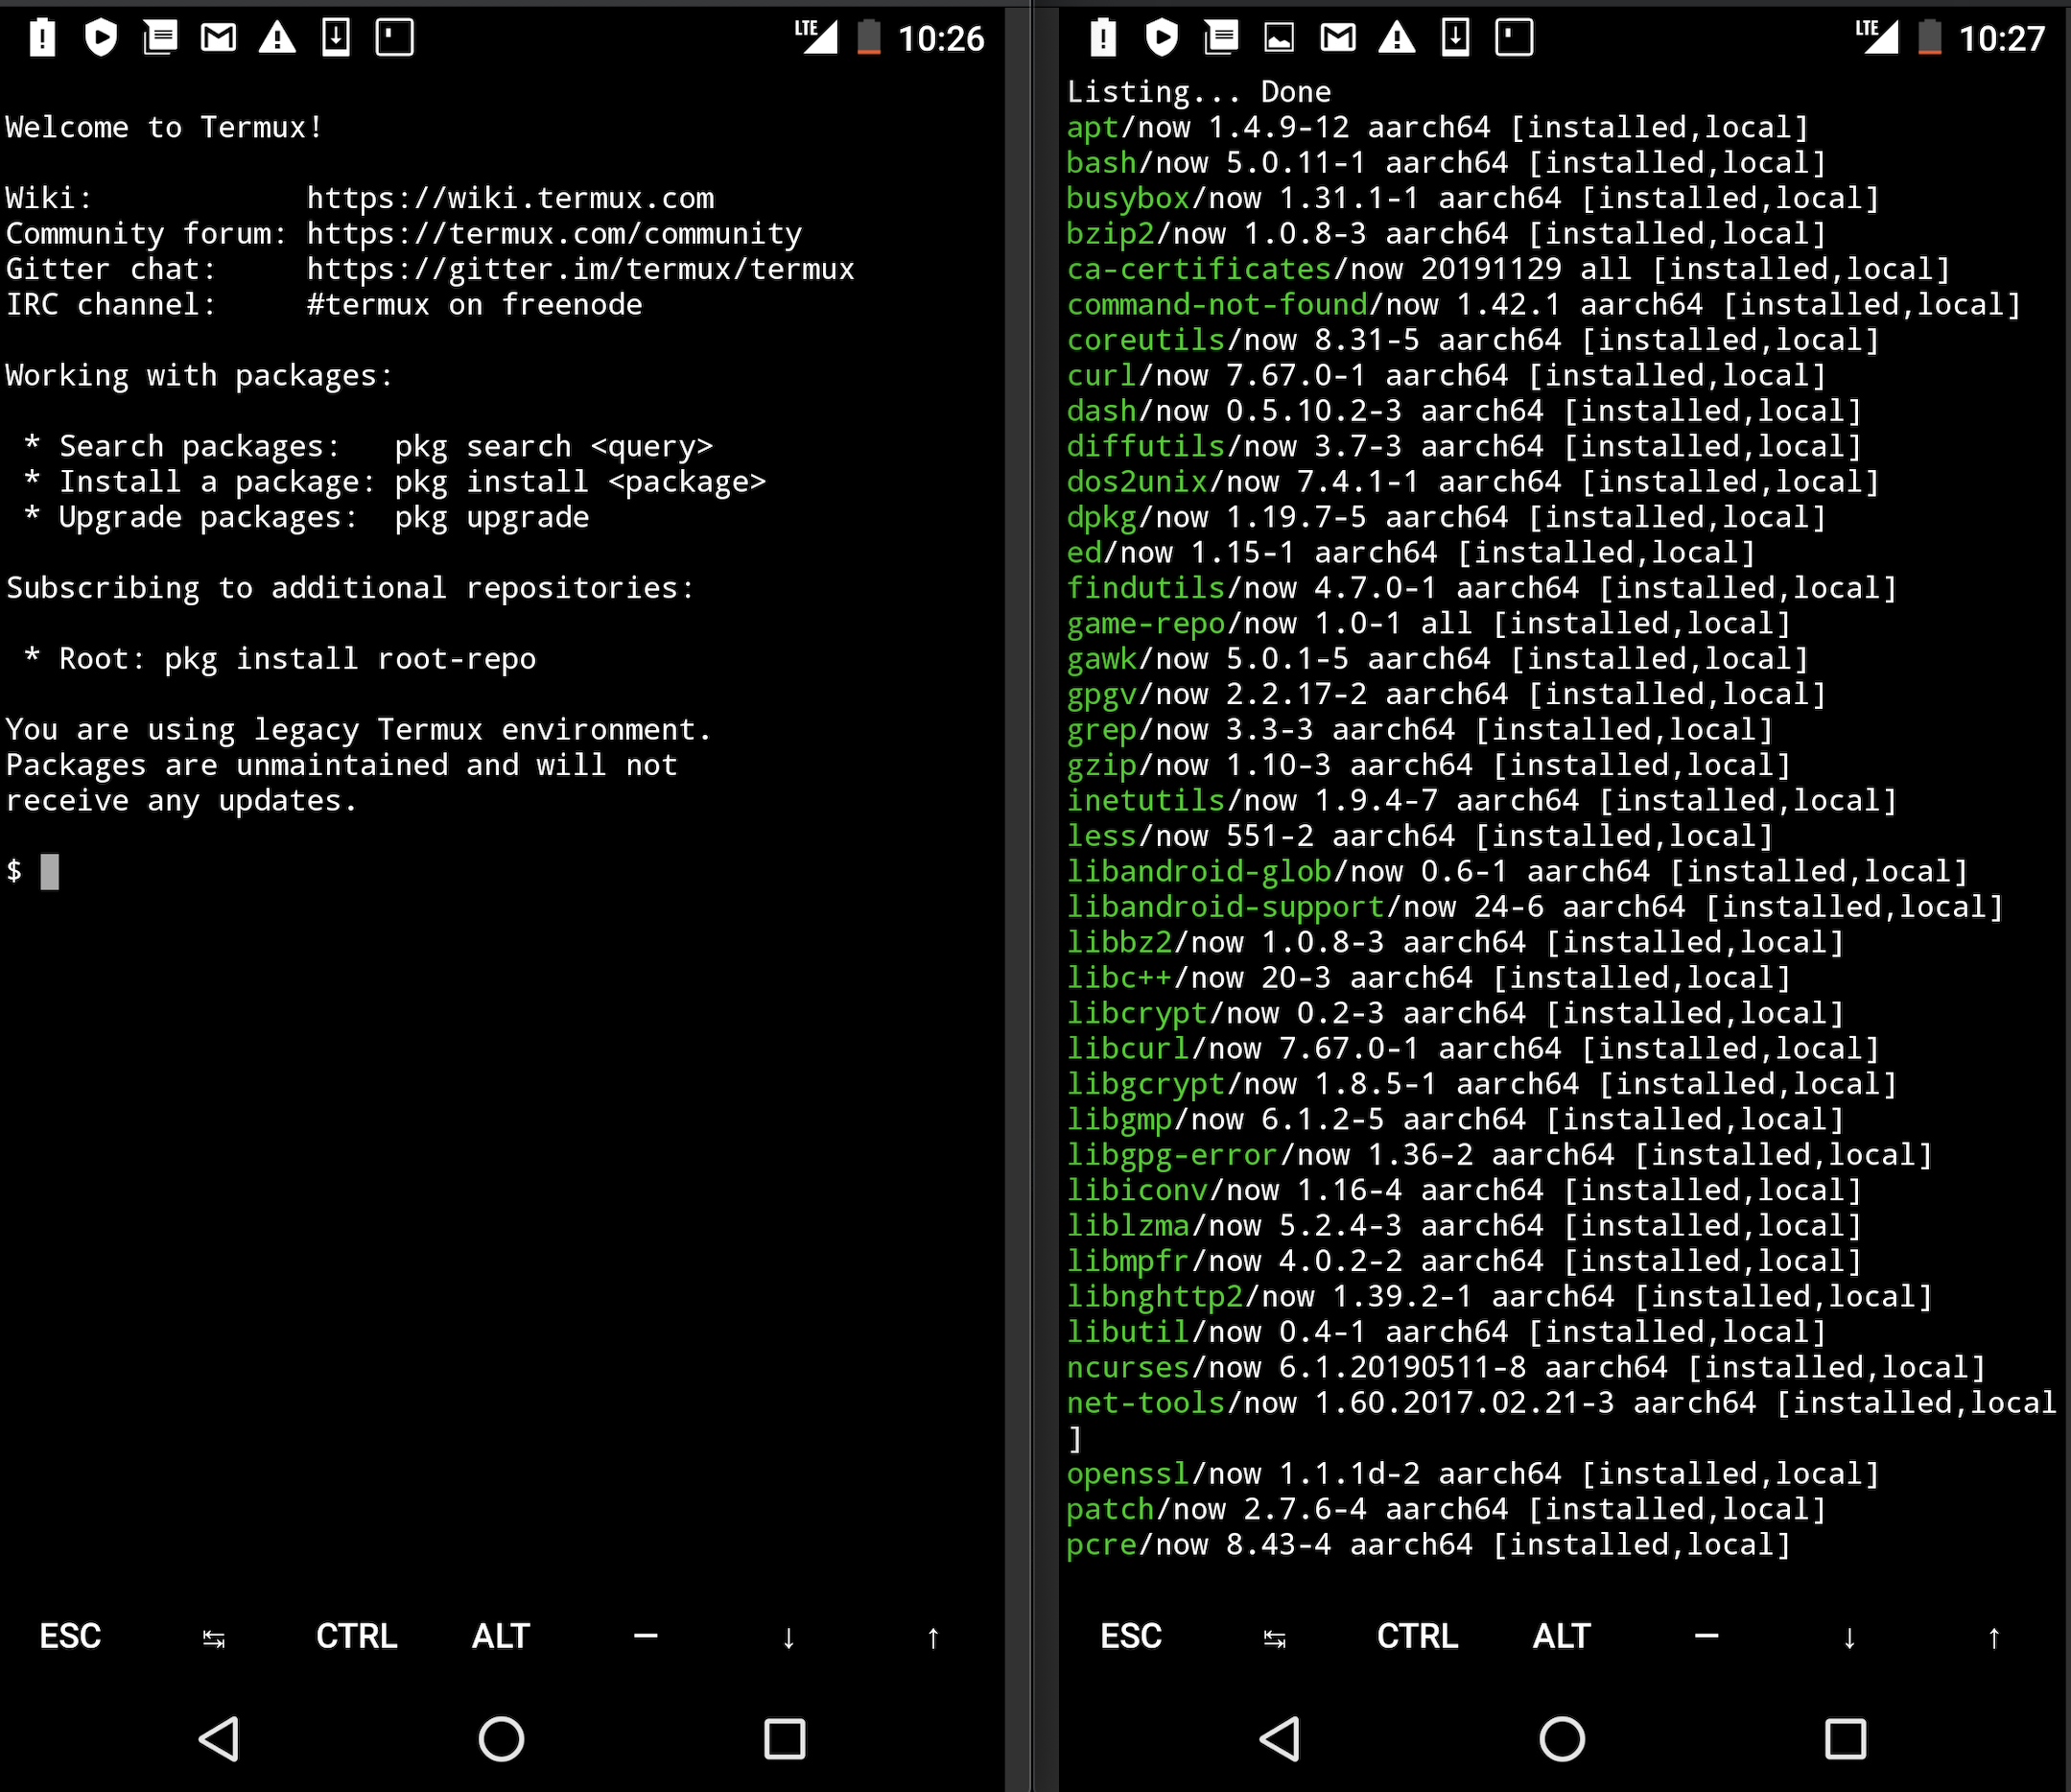
\includegraphics[scale=0.3]{pkg_list_phone}
    \caption{Ported Android pkg manager in Terminal Emulator   }
    \label{fig:pkg_list_phone_12212}
\end{figure}
\vspace{12pt}

\subsection{Implementation of the Control Plane}
The control plane of this hybrid network needs to find the currently available Android devices to change the routing decisions of the network. Previously this was done by allocating a different channel inside the ad hoc network. As ad-hoc networks being are volatile this had bad side effects on the network’s performance. So our proposed method uses a cellular plane as its control channel and Ad hoc network as its data plane.
\\
When an Android device is connected to the Ad-hoc network using the WIFI Direct protocol that device contacts a predefined server creating a reverse ssh connection to that server’s specific port. After that, the server connects back to the Android device using that reverse ssh tunnel bypassing the firewalls and network address translation implemented by the service provider. As the cellular connections use IP pooling the external IP changes in an uneven manner.

\begin{figure}[H]
    \centering
    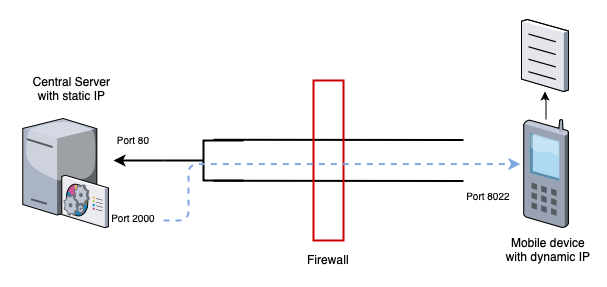
\includegraphics[scale=0.5]{reverse_ssh}
    \caption{Creating a reverse SSH connection between server and the device}
    \label{fig:reverse_ssh_1231313}
\end{figure}
\vspace{12pt}

After connecting to the Android device it finds the IP addresses of the ad-hoc and cellular interfaces. Then it creates a tunnel through the ad-hoc network with the same IP address as the cellular interface of the devices. Then it increases the priority of the tunnel interface using the routing table such that if data is passing to the other android device using the cellular connection previously now it uses the tunnel interface. By doing so we are effectively prioritizing the ad hoc network over the cellular one. If the ad-hoc connections break then tunnel interface is automatically deleted by the bash automation script. So it returns to the normal state.
\begin{figure}[H]
    \centering
    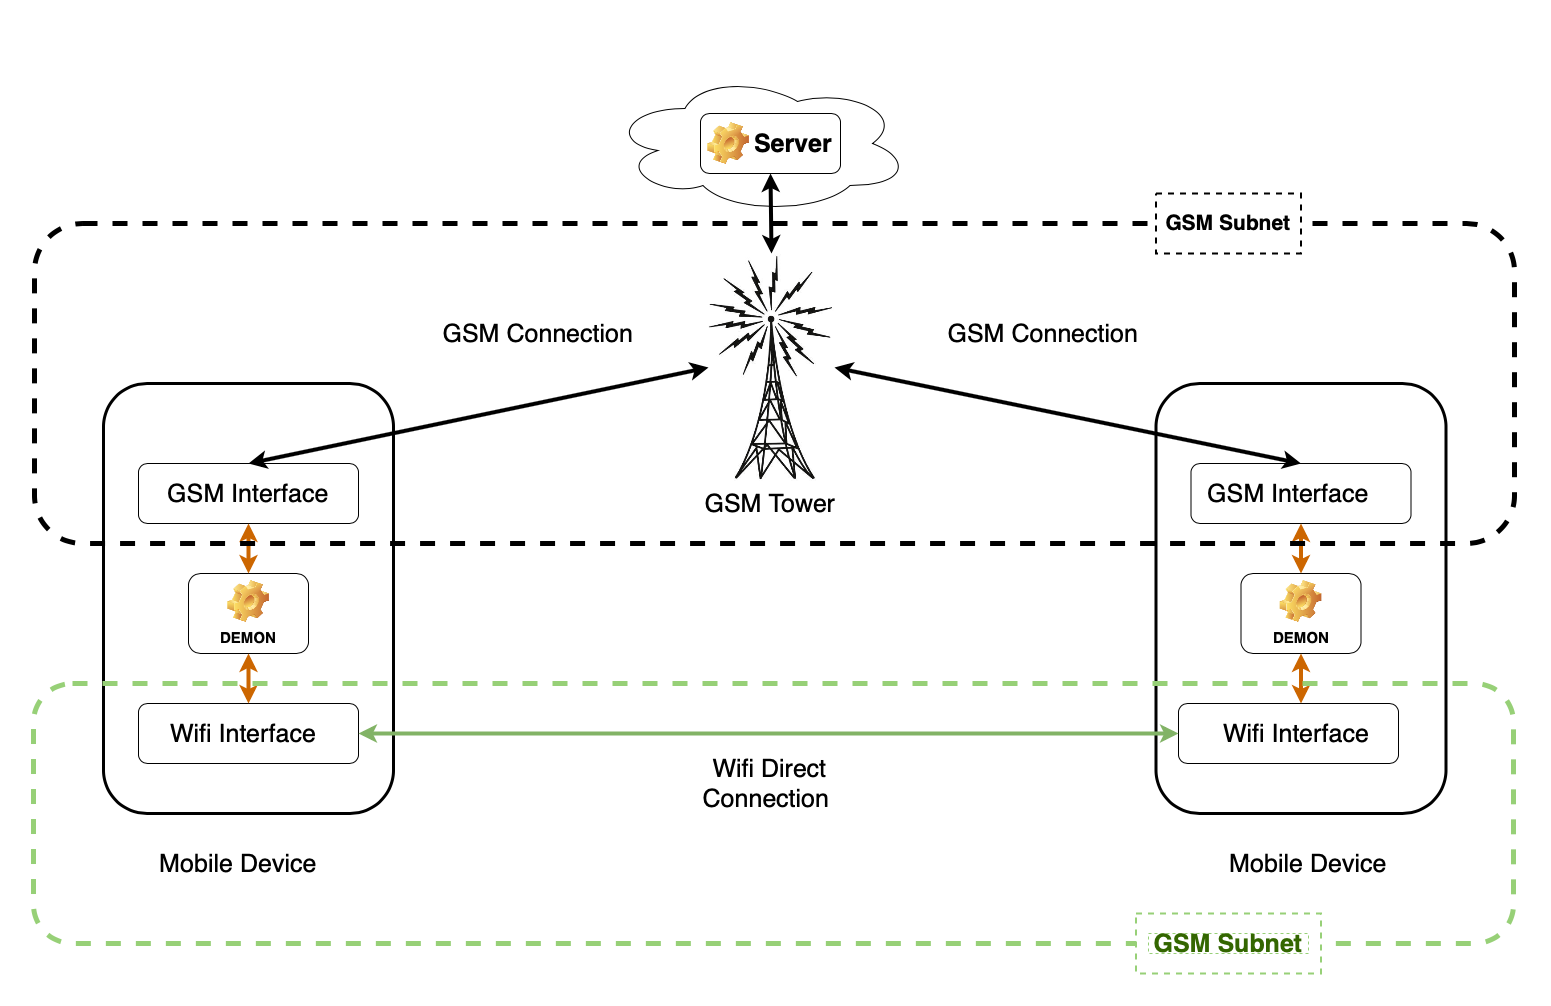
\includegraphics[scale=0.27]{inner_workings_phone_archetecture-2}
    \caption{ High-level Architecture diagram }
    \label{fig:inner_workings_phone_archetecture_23231231231}
\end{figure}
\vspace{12pt}
The IPIP tunnel driver needed to implement this was not natively available in the android kernel. So we had to cross-compile the kerned after adding that module. After doing so we were able to configure the networks of the Android as described above using the remote server in the control plane. As you can see we were able to create a tunnel interface through the ad hoc network by using the IP point to point tunnelling protocol. We gave the external cellular network of device A to the tunnel interface of device B and vice versa. Then we modified the routing table of the Android device to give the newly created tunnel interface a higher priority. Due to this, there are two paths for routing the packets between the android device. Those are the path through the cellular interface and the Ad-hoc interface. As IP tunnel runs through the ad-hoc interface it gets the higher priority. We have implemented the demon process which checks the tunnel connectivity. If the ad-hoc connection breaks it automatically removes the tunnel interface then the Android device comes back to its initial state. 
\begin{figure}[H]
    \centering
    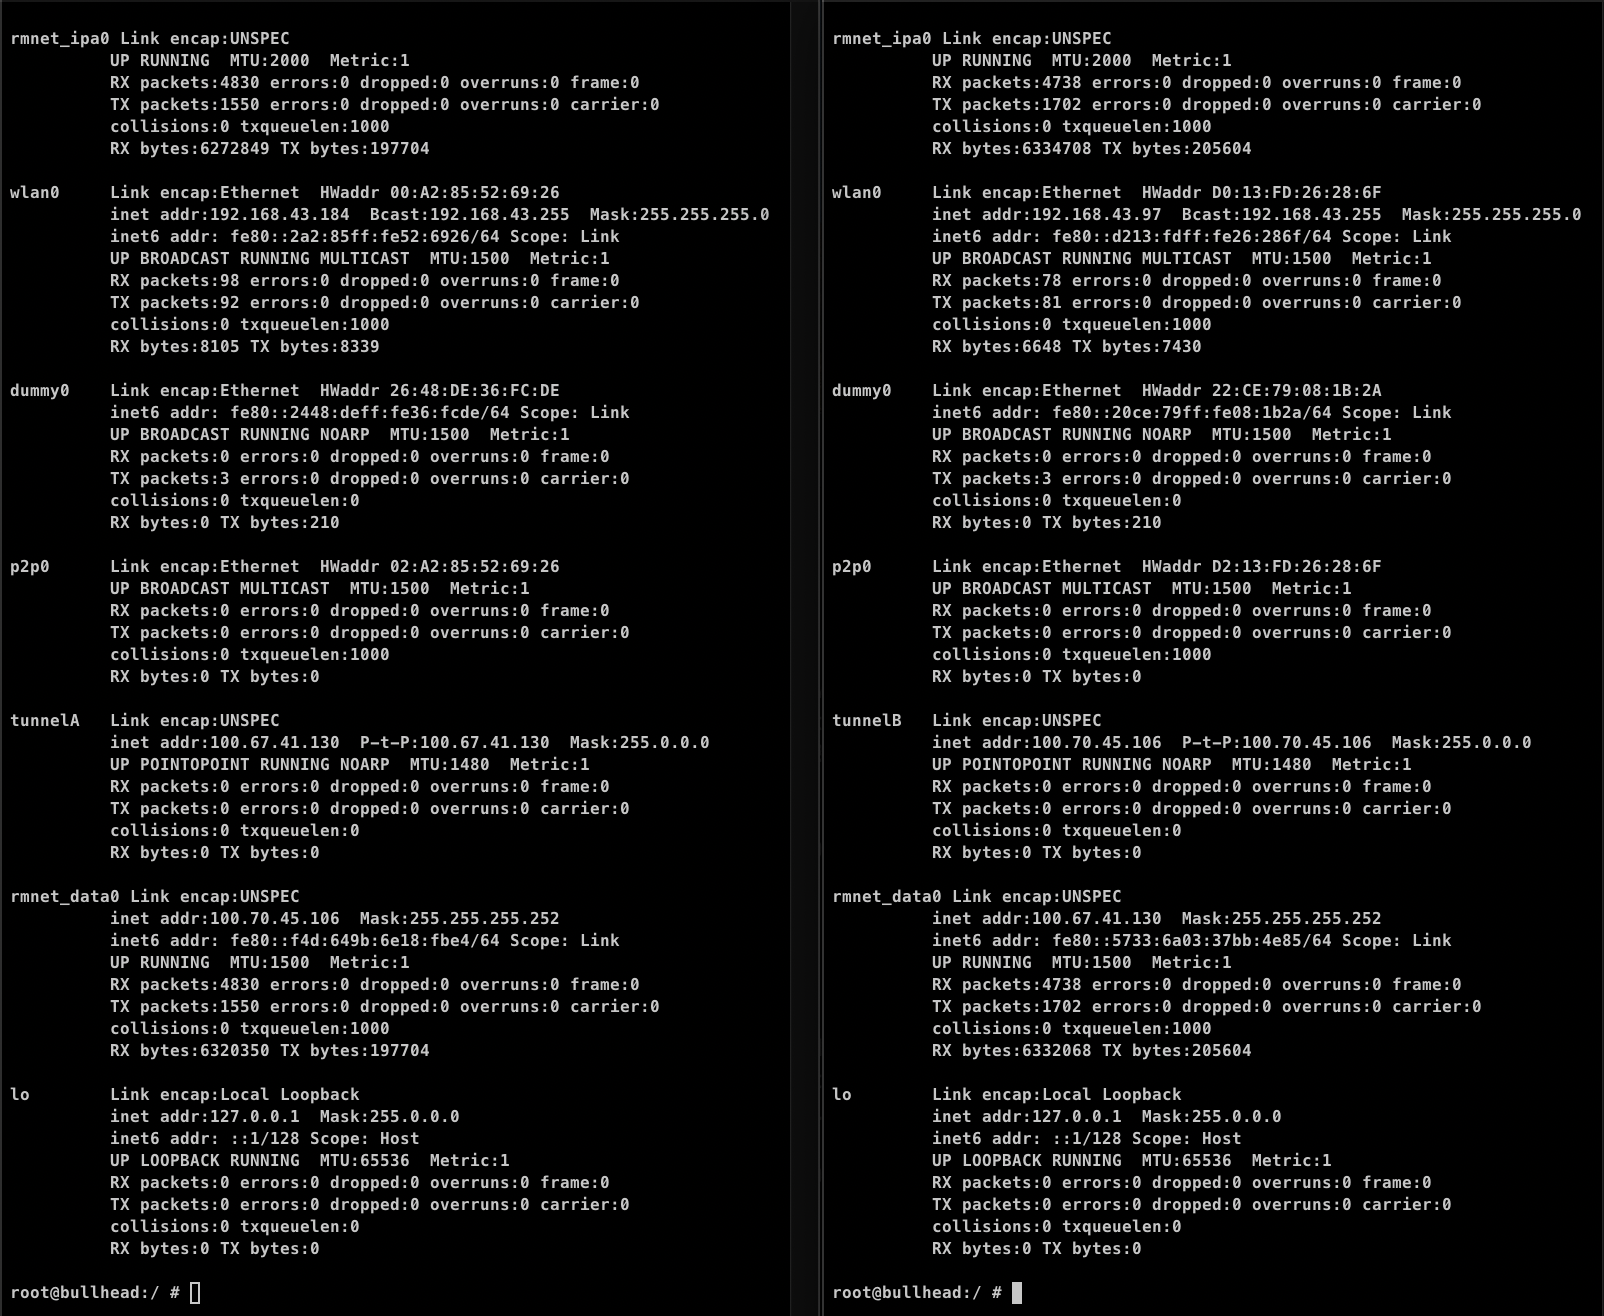
\includegraphics[scale=0.5]{final_result}
    \caption{Final network configurations of two Android devices}
    \label{fig:final_result_2323445}
\end{figure}
\vspace{12pt}

The way that the IP and firewall rules are implemented in the android is not straight forward. So we will be demonstrating this switching process with three Linux machines.









